\section{House of Quality} \label{House of Quality}
HoQ er et værktøj der benyttes i produktudvikling, til at identificere kunders ønsker og krav til det færdige løsning \parencite{Ullman2018TheProcess}. Det skal sikre, at centrale krav identificeres tidligt i processen og omsættes til målbare tekniske parametre, der kan danne grundlag for en struktureret og velbegrundet udviklingsproces. HoQ er opbygget af 8 trin der er illustreret i figur \ref{fig: HOQ illustration}.  

Udarbejdelsen af et HoQ begynder med trin 1, og fortsætter trin for trin. Udover at identificere kundens ønsker og dertilhørende designspecifikationer, skabes der i trin 6 og 8 indsigt i deres indbyrdes sammenhænge og relationer. Dette tydeliggør de designspecifikationer der er vigtigst at fokusere på, samt eventuelle konflikter eller afhængigheder i designet. Det betyder, at ændringen af én designspecifikation har indvirkning på en anden designspecifikation. 

\begin{figure}[H]
    \centering
    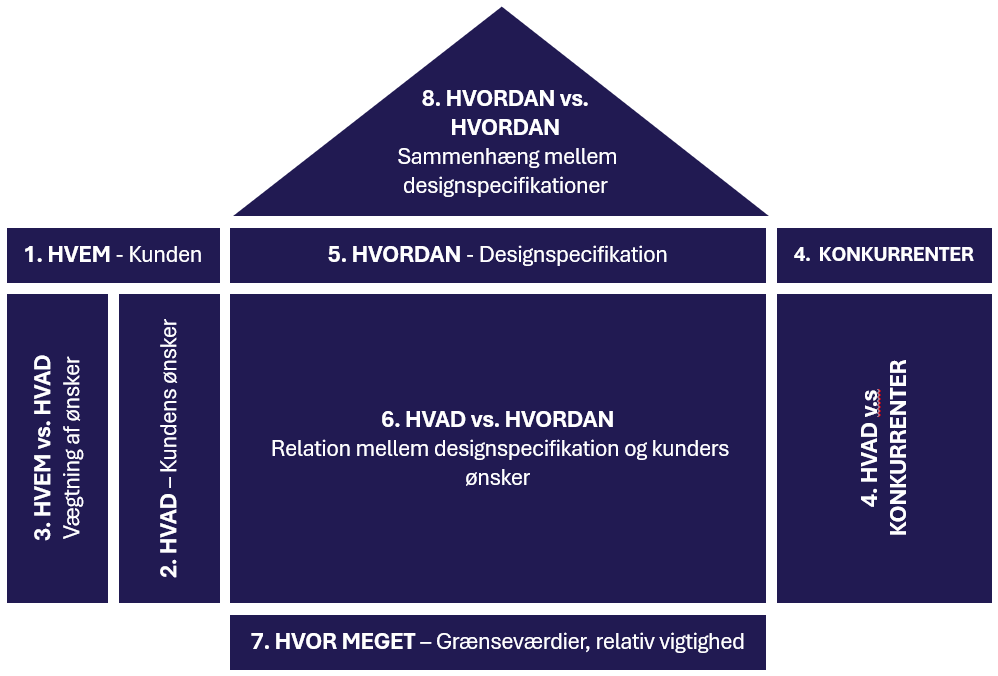
\includegraphics[width=1\linewidth]{Sections/4 Kravspecifikation/Media/HOQ1.png}
    \caption{Illustration af et House of Quality}
    \label{fig: HOQ illustration}
\end{figure} \plainbreak{-0.5}

En væsentlig fordel ved anvendelsen af HoQ er, at metoden bidrager til struktur og systematik i komplekse udviklingsforløb, hvor flere krav og tekniske hensyn skal afvejes. Metoden sikrer desuden en høj grad af klarhed i forhold til, hvordan de opstillede krav afspejles i de valgte designløsninger.



\begin{comment}
\begin{enumerate} 
    \item \textbf{Hvem} - Identifikation af kunder. \\
    \vspace{-0.4cm} \item \textbf{Hvad} - Identifikation af kunders ønsker. \\
    \vspace{-0.4cm} \item \textbf{Hvem vs. hvad} - Vægtning af kundernes ønsker.\\
    \vspace{-0.4cm} \item \textbf{Konkurrenter} - Undersøgelse og evaluering af konkurrenter. \\
    \vspace{-0.4cm} \item \textbf{Hvordan} - Udarbejdelse af designspecifikationer.\\
    \vspace{-0.4cm} \item \textbf{Hvad vs. hvordan} - Relationer mellem designspecifikationer og kundernes ønsker. \\
   \vspace{-0.4cm} \item \textbf{Hvor meget} - Udarbejdelse af grænseværdier for designspecifikationer.\\
\vspace{-0.4cm} \item \textbf{Hvordan vs. hvordan} - Identifikation af designspecifikationernes gensidige afhængighed. \\
\end{enumerate}
\end{comment}

%Processen indledes typisk med en systematisk identifikation af de krav, der vurderes at være væsentlige for det pågældende projekt. Disse krav kan eksempelvis omfatte funktionelle egenskaber, krav til præcision, ydeevne eller andre tekniske specifikationer, der har afgørende betydning for systemets eller produktets samlede funktionalitet. Efterfølgende prioriteres kravene på baggrund af deres betydning, hvorefter de oversættes til konkrete designparametre, som skal sikre opfyldelsen af de ønskede egenskaber.

%HoQ giver et struktureret og visuelt overblik i form af en matrix, hvor relationerne mellem krav og tekniske løsninger tydeliggøres og analyseres. Yderligere skabes der indsigt i, hvordan de tekniske løsninger påvirker hinanden indbyrdes, hvilket muliggør en tidlig identifikation af eventuelle konflikter eller afhængigheder i designet. Herved styrkes beslutningsgrundlaget for udviklingsteamet, som kan foretage prioriteringer med udgangspunkt i en helhedsorienteret vurdering af projektets krav og mål.

%Sammenfattende er HoQ et redskab til at strukturere og kvalificere beslutningsprocesser i projekter, hvor der stilles krav om høj funktionalitet, kvalitet og ydeevne. Metoden giver et solidt fundament for at sikre, at centrale krav bliver integreret i designet, og at de tekniske løsninger udvælges på et velunderbygget grundlag.

